

\begin{frame}[fragile]{Verzweigungen: allgegenwärtig}
    \begin{itemize}[<+->]
        \item Promotionsentscheid (Notendurchschnitt)
              \only<1>{\begin{figure}[H]
                      \centering
                      \begin{tikzpicture}[transform shape, scale=.7, on grid, ->]
                          \tikzstyle{every node}=[font=\small]
                          % grid to easier see that the node centers line up while developing plot
                          %\draw [help lines] (-5,-9) grid (9,1);
                          \node (start) [code] {\lstinline|note_schnitt = 3.6|};
                          \node (dec1) [decision, below=2.5cm of start] {\lstinline|note_schnitt >= 3.75|};
                          \node (printif) [code, below left=1.5cm and 4cm of dec1] {\lstinline|print("Semester bestanden")|};
                          \node (printelse) [code, below right=1.5cm and 4cm of dec1] {\lstinline|print("Semester nicht bestanden")|};
                          \node (end) [circle,draw=black, fill=black, below=3cm of dec1] {};

                          \draw (start) -- (dec1);
                          \draw (dec1) -| node[anchor=top, above=.1cm] {\lstinline|True|} (printif);
                          \draw (dec1) -| node[anchor=top, above=.1cm] {\lstinline|False|} (printelse);
                          \draw (printif) |- (end);
                          \draw (printelse) |- (end);

                      \end{tikzpicture}
                  \end{figure}}
        \item Wie gehe ich zur Schule?
              \only<2>{\begin{figure}[H]
                      \centering
                      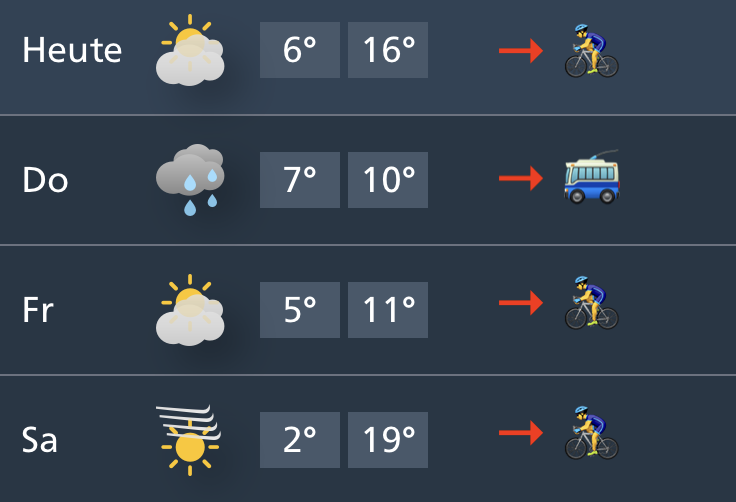
\includegraphics[width=0.7\linewidth]{GrundlagenInfo/00_Programmieren/Figures/if-elif-else-weather}
                  \end{figure}
                  $\rightarrow$ \textit{und wenn ich gesund bin / mich bewegen kann}}
        \item Medizinische Entscheide
              \only<3>{\begin{figure}[H]
                      \centering
                      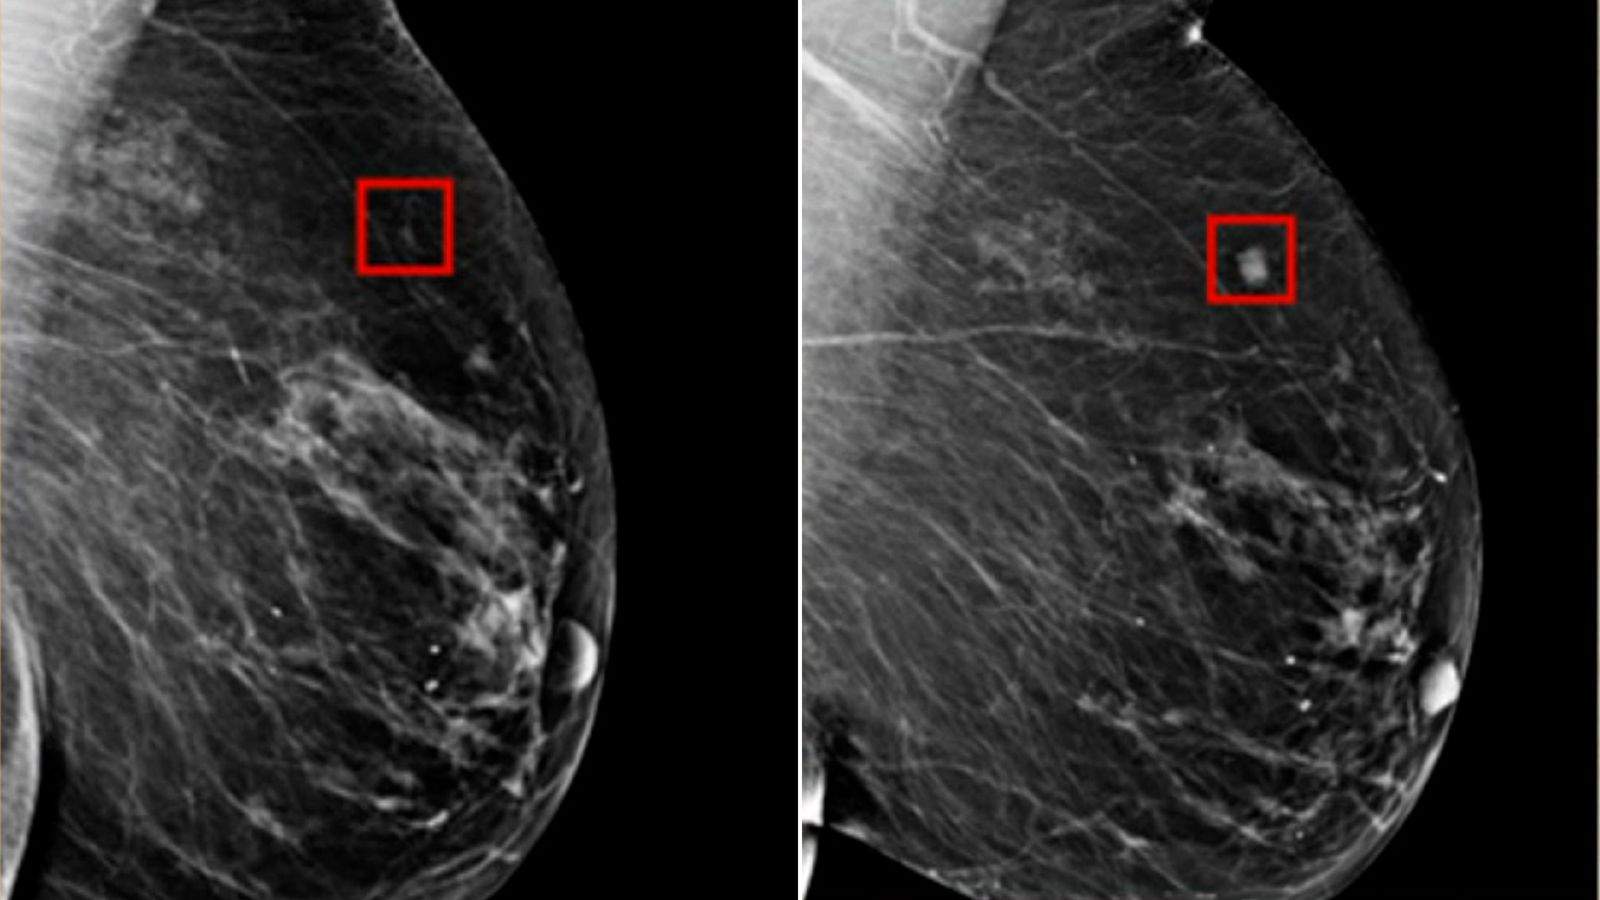
\includegraphics[width=0.7\linewidth]{GrundlagenInfo/00_Programmieren/Figures/if-elif-else-cancer}
                  \end{figure}
                  $\rightarrow$ \textit{Und wenn die Fachärzte dies bestätigen}}
        \item Etc.
    \end{itemize}
\end{frame}
